% Relatório do Trabalho IV — Sistemas Operacionais (FURG), no modelo SBC (sbc-template.sty / sbc.bst).
% Compilar:  latexmk -pdf relatorio.tex   (usa BibTeX com relatorio.bib)
\documentclass[12pt]{article}

\usepackage{graphicx,url}
\usepackage[T1]{fontenc}
\usepackage[utf8]{inputenc}
\usepackage[brazilian]{babel}
\usepackage{sbc-template}
\usepackage{array}
\usepackage{placeins}
\usepackage[hidelinks]{hyperref}

\hypersetup{
  pdftitle={Custo de desempenho da ofuscação de código Python},
  pdfauthor={Pedro Machado, Marcos Freitas e Alexsander Santos}
}

\setlength{\tabcolsep}{3pt}
\sloppy

\title{Custo de desempenho da ofuscação de código Python: um estudo com PyArmor e python-minifier em três máquinas}

\author{Pedro Machado\inst{1}, Marcos Freitas\inst{1},
  Alexsander Santos\inst{1}}

\address{Universidade Federal do Rio Grande (FURG)\\
  Rio Grande -- RS -- Brasil
  \email{pedro.machado@furg.br, mcopellofreitas@hotmail.com}
  \email{alexsander.oml@gmail.com}
}

\begin{document}

\maketitle

\begin{abstract}
We measured the execution-time cost of Python obfuscation with matrix multiplication and word counting.
The experiment compared the original programs, python-minifier and two PyArmor trial configurations on
three machines, with three input sizes and ten repetitions per case. Mean runtimes stayed close to the
original for python-minifier. PyArmor increases were more consistent on Pedro's machine, ranging from
1.8\% to 8.3\%. Across the tested inputs, relative costs showed no consistent increase with input size.
These results describe the tested configurations and do not measure resistance to reverse engineering.
\end{abstract}

\begin{resumo}
Medimos o custo de tempo da ofuscação de código Python com multiplicação de matrizes e contagem de palavras.
Comparamos os programas originais, o \emph{python-minifier} e duas configurações do PyArmor \emph{trial} em três
máquinas, com três tamanhos e dez repetições por caso. As médias do \emph{minifier} ficaram próximas às do
original. Os aumentos com PyArmor foram mais consistentes na máquina do Pedro, variando de 1,8\% a 8,3\%.
Nas entradas testadas, o custo relativo não apresentou aumento consistente com o tamanho. Os resultados
se limitam às configurações avaliadas e não medem a resistência à engenharia reversa.
\end{resumo}


\section{Introdução}
A ofuscação é uma camada de defesa: não impede o acesso ao código, mas aumenta o esforço necessário para
compreendê-lo e manipulá-lo. O enunciado propõe investigar o compromisso entre o custo computacional e a dificuldade de analisar o código. O objetivo deste trabalho é \emph{medir} esse custo: quanto
mais lento fica um programa Python depois de ofuscado, e se esse custo depende do benchmark, do tamanho da
entrada e da máquina. A base de comparação é sempre o código Python \textbf{não ofuscado}, na mesma máquina.

Os dois benchmarks são os fornecidos pelo professor e não foram modificados: \textbf{matrizes} (multiplicação
$n\times n$ com três laços aninhados, custo $O(n^3)$) e \textbf{palavras} (contagem de frequência de $n$ palavras
em um dicionário, custo médio esperado $O(n)$). Cada programa imprime o tempo da parte computacional (\texttt{time: X seconds}) e
verifica a própria saída; esse é o tempo usado em todas as análises.

\section{Ambiente de teste}
Cada integrante rodou o mesmo procedimento na própria máquina (Tabela~\ref{tab:amb}). Todas são desktops
(sem bateria); programas foram fechados, a suspensão foi desativada e a máquina ficou sem uso durante a rodada,
conforme confirmação registrada por cada integrante antes de iniciar. A frequência efetiva da CPU não foi
monitorada. Como SO, CPU, versão do Python e perfil de energia mudam \emph{juntos} entre as máquinas, diferenças
entre elas não podem ser atribuídas a uma única causa.

\begin{table}[!htbp]\centering\scriptsize\setlength{\tabcolsep}{3pt}
\caption{Máquinas usadas. Todas com PyArmor 9.2.8 (\emph{trial}) e python-minifier 3.4.0.}\label{tab:amb}
\begin{tabular}{lccc}\hline
 & Pedro & Alex & Marcos \\\hline
SO & Windows 10 (build 19045) & Ubuntu 26.04.1 (kernel 7.0.0) & Fedora 44 (kernel 7.2.15) \\
CPU & Intel i7-9700 & Intel Xeon E-2124 & AMD Ryzen 5 5500 \\
Núcleos/\emph{threads} & 8/8 & 4/4 & 6/12 \\
RAM & 31,9 GiB & 30,6 GiB & 15,5 GiB \\
Python (CPython) & 3.12.15 & 3.13.7 & 3.14.10 \\
Energia/\emph{governor} & alto desempenho & \texttt{powersave}, \emph{turbo} ativo & \texttt{powersave} \\
Tamanhos de matrizes & 560, 840, 1264 & 560, 840, 1264 & 608, 912, 1368 \\
Execução da rodada & 04/11 23:58 -- 05/11 05:48 & 05/11 07:20 -- 12:13 & 05/11 01:14 -- 06:36 \\\hline
\end{tabular}
\end{table}
As versões de Python e do kernel na tabela seguem o manifesto da execução. O arquivo de preparação
\texttt{resultados/marcos/sistema.md} é anterior à rodada e registra Python 3.14.8 e kernel 7.2.11.

\section{Configurações de ofuscação}
Além do original, foram usadas três configurações (Tabela~\ref{tab:cfg}).

\begin{table}[!htbp]\centering\footnotesize
\caption{Configurações de ofuscação (\texttt{scripts/ofuscar.py} as gera a partir de \texttt{src/}).}\label{tab:cfg}
\begin{tabular}{p{3.1cm}p{3.6cm}>{\raggedright\ttfamily\scriptsize\arraybackslash}p{7.2cm}}\hline
configuração & técnicas & comando \\ \hline
minifier-renomear & renomeação de identificadores; remoção de comentários e \emph{docstrings} &
pyminify --rename-globals --output SAÍDA ENTRADA \\[3pt]
pyarmor-basico & empacotamento e criptografia do bytecode; \emph{runtime} nativo &
pyarmor gen -O SAÍDA ENTRADAS \\[3pt]
pyarmor-forte & o anterior $+$ \texttt{jit}, modo privado e asserções &
pyarmor gen --obf-module 1 --obf-code 1 --enable jit --private --assert-call --assert-import -O SAÍDA ENTRADAS \\ \hline
\end{tabular}
\end{table}
Segundo \texttt{pyarmor gen --help}, \texttt{--obf-module 1} e \texttt{--obf-code 1} já são o padrão; logo, a diferença
do ``forte'' para o ``básico'' é \texttt{jit}, \texttt{private} e as asserções.
A licença \emph{trial} do PyArmor recusa \texttt{--obf-code 2}, \texttt{--mix-str} e \texttt{--enable rft|bcc}
(\texttt{out of license}); o nome ``forte'' identifica a combinação adicional escolhida, sem representar uma medida de proteção.

\textbf{Instalação.} Python~3 com ambiente virtual e as duas ferramentas fixadas em \texttt{requirements.txt}:
\texttt{python3 -m venv .venv; source .venv/bin/activate; pip install -r requirements.txt}
(\texttt{pyarmor==9.2.8} \cite{pyarmor}, \texttt{python-minifier==3.4.0} \cite{pyminifier}). Cada máquina gera o próprio diretório
\texttt{ofuscado/<id>/}, pois o \emph{runtime} do PyArmor depende de SO, arquitetura e versão do Python.

\section{Metodologia}
\textbf{Tamanhos.} Três entradas por benchmark, com crescimento de pelo menos 50\% entre tamanhos consecutivos: matrizes
560/840/1264 (Marcos: 608/912/1368, por margem sobre 20~s) e palavras 50M/80M/128M. A menor entrada do
original em matrizes ficou entre 22,7 e 26,7~s nas três máquinas ($\ge 20$~s).
\textbf{Exceção em palavras:} o programa guarda todo o corpus na RAM (pico de 6,7~GiB no maior caso do Marcos, que tem 15,5~GiB de RAM), e chegar a
20~s exigiria entradas que não cabem na memória. O professor, consultado por um integrante, respondeu que o
mínimo de 20~s pode ser flexibilizado para este benchmark. Essa orientação recebida em conversa com o grupo está registrada (04/11/2026) em
\texttt{config.json}. A menor entrada de palavras do original levou de 3,1 a 4,2~s.

\textbf{Repetições.} Dez por caso (4 configurações $\times$ 3 tamanhos $\times$ 2 benchmarks $\times$ 10 =
240 execuções por máquina), \emph{intercaladas} entre configurações. Todas as 720 execuções terminaram com saída
correta e código de retorno zero; uma auditoria automática (\texttt{scripts/auditar.py}) aprovou as três rodadas
sem erros ou avisos.

\textbf{Estatísticas.} Média, mediana, desvio padrão amostral, mínimo e máximo (tabelas completas no Apêndice
e Figura~\ref{fig:stats}). O \textbf{slowdown} é a média ofuscada dividida pela média do original, no mesmo
tamanho e máquina. Como análise complementar, estimamos intervalos de 95\% do slowdown por
\emph{bootstrap}, com 5000 reamostragens independentes das dez repetições de cada configuração.
Um intervalo que inclui 1,0 é compatível com ausência de diferença entre as médias. Esses intervalos
são exploratórios, sem ajuste para as várias comparações, e não demonstram equivalência entre programas.

\section{Resultados}
A Tabela~\ref{tab:resumo} resume o maior tamanho de cada máquina e a Figura~\ref{fig:slow} mostra o slowdown em
todos os tamanhos. As cinco estatísticas por máquina estão na Figura~\ref{fig:stats} e nas tabelas completas do Apêndice.

\begin{table}[ht]\centering\footnotesize
\caption{Slowdown (média ofuscada / média original) no maior tamanho, com IC 95\% por bootstrap. Negrito: IC não contém 1,0.}\label{tab:resumo}
\begin{tabular}{llccc}\hline
benchmark & máquina (tamanho) & minifier-renomear & pyarmor-basico & pyarmor-forte \\\hline
matrizes & Pedro (1264) & 1,002 [0,987; 1,019] & \textbf{1,033 [1,022; 1,046]} & \textbf{1,029 [1,017; 1,040]} \\
matrizes & Alex (1264) & 1,004 [0,998; 1,010] & 0,999 [0,995; 1,002] & 0,999 [0,995; 1,003] \\
matrizes & Marcos (1368) & 0,997 [0,982; 1,009] & 1,014 [0,980; 1,058] & 0,992 [0,978; 1,004] \\
palavras & Pedro (128M) & 1,001 [0,971; 1,032] & \textbf{1,048 [1,020; 1,079]} & \textbf{1,050 [1,018; 1,082]} \\
palavras & Alex (128M) & \textbf{0,972 [0,954; 0,991]} & 1,002 [0,982; 1,022] & 0,993 [0,975; 1,010] \\
palavras & Marcos (128M) & \textbf{0,962 [0,934; 0,988]} & \textbf{0,968 [0,938; 0,996]} & \textbf{0,973 [0,945; 0,999]} \\
\hline\end{tabular}\end{table}


\begin{figure}[!htbp]\centering
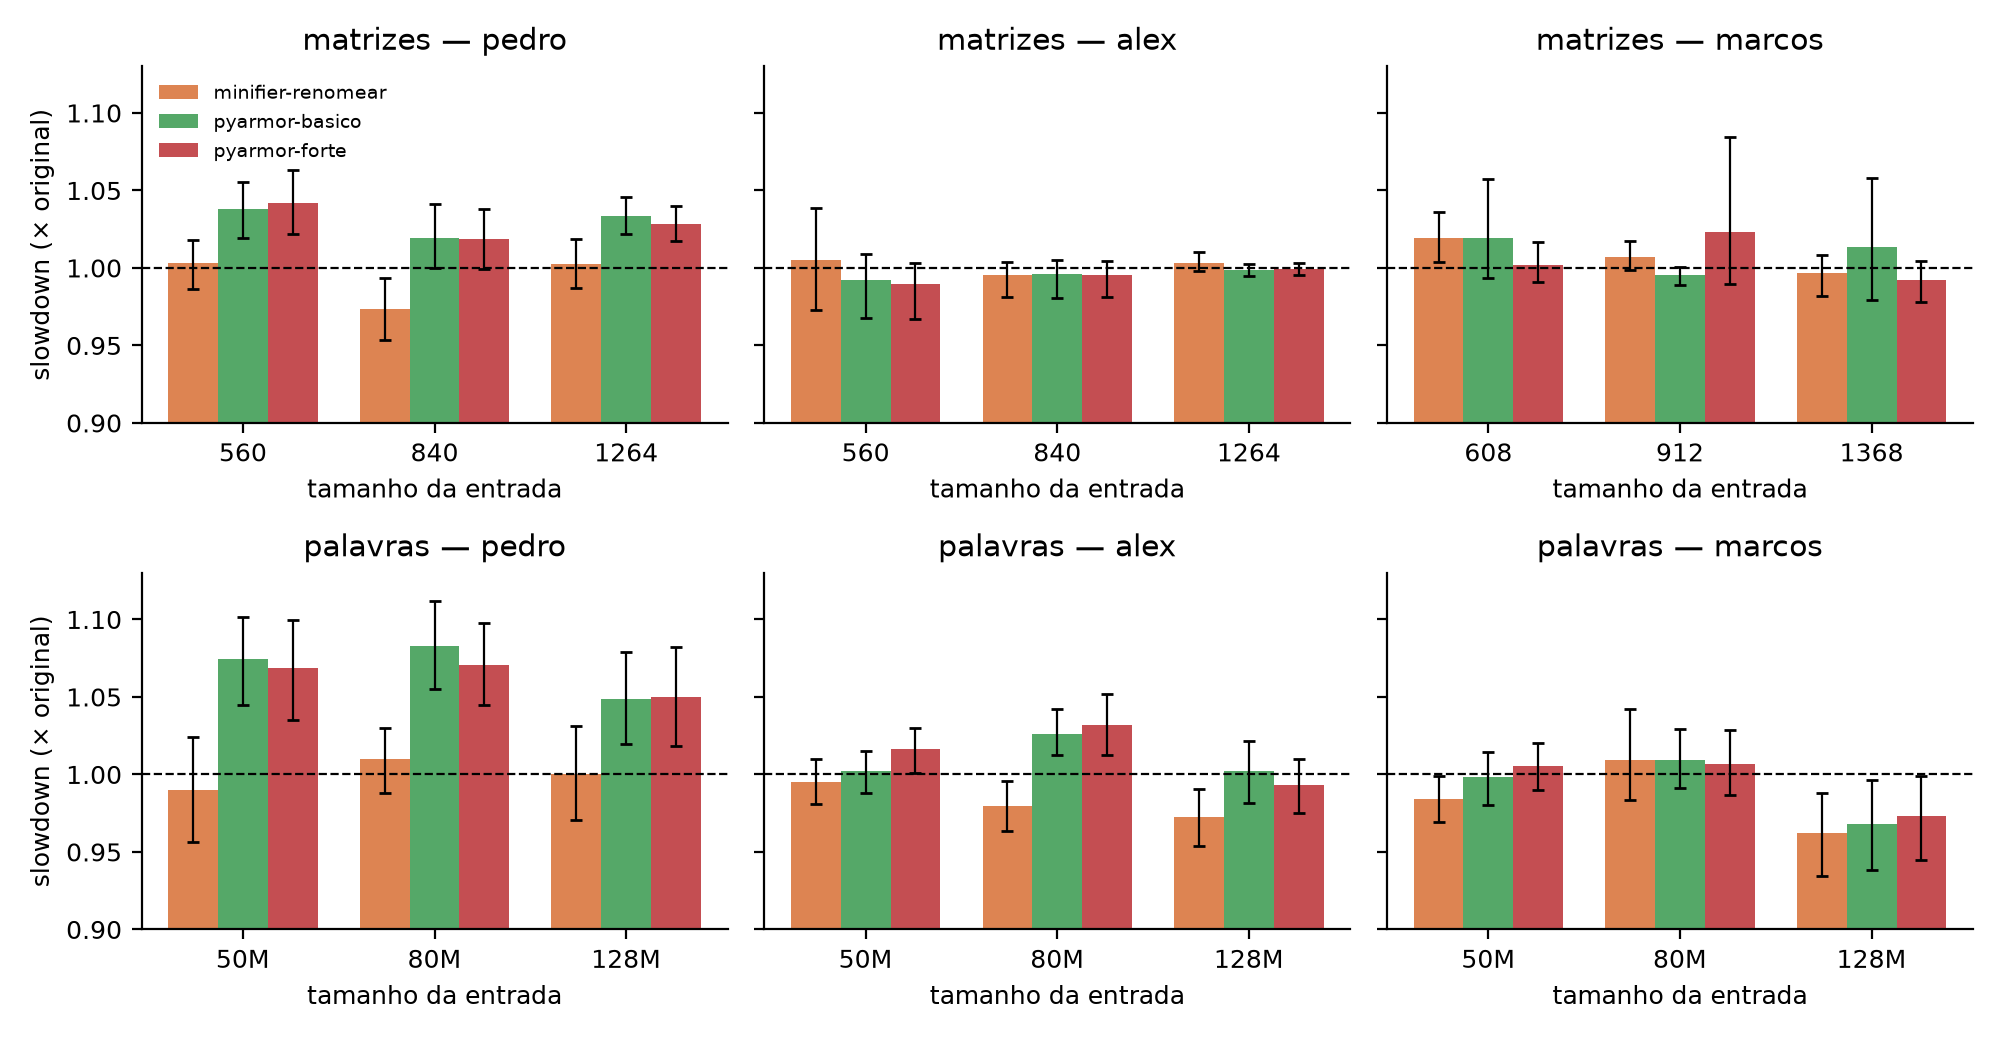
\includegraphics[width=\textwidth]{fig/slowdown.png}
\caption{Slowdown de cada configuração em relação ao original (linha tracejada = 1,0), com IC 95\% por \emph{bootstrap}.}\label{fig:slow}
\end{figure}

\section{Análise}

\begin{figure}[!htbp]\centering
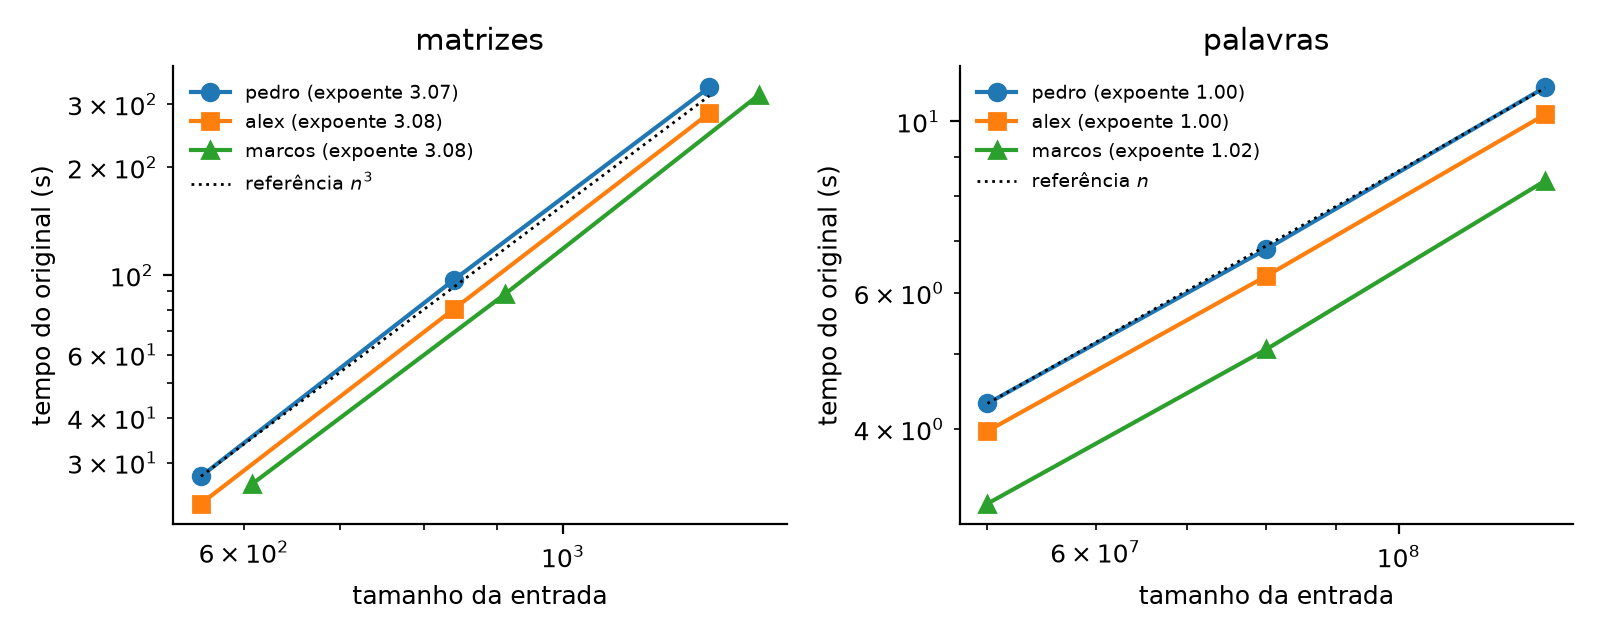
\includegraphics[width=0.85\textwidth]{fig/escalonamento.png}
\caption{Tempo do código original em função do tamanho, em escala log-log. O expoente usa o menor e o maior tamanho.}\label{fig:esc}
\end{figure}

\textbf{Crescimento com a entrada.} Nos originais, o expoente medido entre o menor e o maior tamanho
foi de 3,07 a 3,08 em matrizes e de 1,00 a 1,02 em palavras (Figura~\ref{fig:esc}). Esses valores são próximos
às ordens esperadas de crescimento. Em matrizes, o tempo por iteração do laço interno aumentou cerca de
6\% entre os extremos. Não coletamos contadores de cache ou frequências durante a rodada para explicar
esse aumento. O slowdown das versões ofuscadas não apresentou tendência consistente de crescimento
nos três tamanhos avaliados (Figura~\ref{fig:slow}). O maior valor observado foi 1,083$\times$.

\textbf{Diferenças entre configurações.} O \emph{python-minifier} apresentou slowdowns de 0,96 a 1,02.
Seis dos 18 intervalos estimados não incluem 1,0, com diferenças em ambos os sentidos. Portanto, os dados
não sustentam um ganho ou uma perda uniforme de desempenho com essa configuração. As transformações
visíveis no código incluem renomeação e remoção de metadados, mantendo a estrutura dos laços apresentada
na Figura~\ref{lst:min}. Não comparamos o bytecode para atribuir a essas transformações um custo exato.

Na máquina do Pedro, as médias com PyArmor aumentaram de 1,8\% a 4,2\% em matrizes e de 4,8\% a 8,3\% em
palavras. Dez dos 12 intervalos correspondentes ficaram acima de 1,0. Nas outras máquinas, os valores
ficaram mais próximos de 1,0 e algumas médias foram menores que as do original. Como CPU, SO, Python e
perfil de energia variam juntos, o experimento não identifica a causa dessas diferenças.

\textbf{PyArmor básico e forte.} As médias das duas configurações ficaram próximas, com diferenças de
até 2,8 pontos percentuais no slowdown. Esse resultado descreve os programas e opções testados. Não fizemos
um teste de equivalência nem isolamos o efeito de \texttt{jit}, modo privado e asserções. Também não
medimos a resistência de cada configuração à análise do código.

\textbf{Variação entre repetições.} Alguns casos do Marcos tiveram execuções mais longas: 366,6~s no
PyArmor básico com $n=1368$ (mediana de 312,0~s) e 114,3~s no forte com $n=912$ (mediana de 88,1~s).
Essas observações permanecem nas dez amostras e afetam a média e o desvio. Pelas medianas, os slowdowns
desses casos são 0,990 e 0,997. Não há uma margem única, como 3\%, que separe efeito e variação em todos
os casos. A dispersão e os intervalos devem ser lidos junto das médias.

\textbf{Tempo total e tempo computacional.} Em matrizes, a diferença entre o tempo total do processo e
o tempo interno ficou entre 0,06 e 0,22~s nas médias dos casos. Em palavras, ficou aproximadamente entre
6 e 19~s. O programa constrói o corpus antes do cronômetro, de modo que essa diferença inclui a preparação
da entrada, além da inicialização do Python, do carregamento do código e de outros custos do processo.
A medição não separa essas parcelas e não permite atribuir toda a diferença ao PyArmor.

\textbf{Comparação entre máquinas.} Em palavras com 128 milhões de elementos, a média do original foi
11,1~s no Pedro, 10,2~s no Alex e 8,4~s no Marcos. Em matrizes, os maiores tamanhos diferem entre as máquinas,
como indicado na Tabela~\ref{tab:resumo}. O slowdown compara cada configuração ao seu próprio original,
mas não elimina as diferenças de tamanho, hardware, interpretador ou energia entre participantes.

\textbf{Segurança e desempenho.} O enunciado apresenta a ofuscação como uma forma de dificultar a análise
do código. A discussão de segurança por obscuridade e do princípio de Kerckhoffs ajuda a delimitar essa
proteção \cite{kerckhoffs1883,tanenbaum2016}. Aqui avaliamos apenas o custo de tempo. O trecho do
\emph{minifier} ainda permite acompanhar os laços e os índices. O PyArmor usa um arquivo de inicialização
e um \emph{runtime} nativo. Essas diferenças não medem quanto tempo um analista precisaria para compreender
ou recuperar o programa.

\section{Dificuldades e decisões}
\begin{itemize}
\item \textbf{PyArmor \emph{trial}.} Recusa \texttt{--obf-code 2}, \texttt{--mix-str}, \texttt{--enable rft|bcc}
(\texttt{out of license}). Decisão: a config ``forte'' usa só o que a \emph{trial} aceita.
\item \textbf{Duração de palavras.} Os tamanhos globais foram definidos na máquina de referência e não chegam
a 20~s em palavras (a primeira rodada do Pedro, em 28--29/10, antes do pré-voo revisado, já mostrou isso: 4,3 a 10,9~s).
Aumentar só a entrada exigiria extrapolar para ${\sim}$234M--527M palavras, ${\sim}$34~GiB de RAM livre no Pedro. Foi
preparado um perfil de CPU a 1200~MHz para alongar o cálculo, mas \textbf{não foi usado}. Decisão final: manter
os tamanhos e adotar a exceção aceita pelo professor (piso de 1~s). Aquela primeira rodada foi descartada e a
rodada de 04--05/11 usa o pré-voo revisado (mede os dois menores originais e o pico de RAM do maior palavras).
\item \textbf{Pedro:} a instalação mostrou \texttt{WARNING: Cache entry deserialization failed, entry ignored}, sem impedir a instalação ou a execução.
\item \textbf{Alex:} a primeira instalação falhou por rede restrita (\texttt{Could not find a version that satisfies
the requirement pyarmor==9.2.8}); resolvida com acesso externo. Usou Python 3.13.7 (o padrão do sistema é 3.14.4)
por compatibilidade com o \emph{runtime}; a geração em 3.14 não foi testada por ele.
\item \textbf{Marcos:} o pré-voo de 03/11 reprovou o maior palavras por RAM livre insuficiente ou não medida (15,5~GiB de RAM);
a rodada de 05/11 foi aprovada no pré-voo (pico de 6,7~GiB). Usou matrizes 608/912/1368 por margem sobre 20~s.
\item \textbf{Retomada.} O executor registra Python, fontes, configuração e perfil e recusa retomar com
condições diferentes; assim as amostras de uma máquina não se misturam.
\item \textbf{Limitações.} Frequência da CPU não monitorada; três máquinas diferem em várias variáveis; apenas dez
repetições por caso. Os intervalos variam conforme o caso e não estabelecem um limite geral de detecção de efeitos.
\end{itemize}

\section{Extras}
\textbf{Mais de um sistema:} Windows, Ubuntu e Fedora, com Python 3.12, 3.13 e 3.14.
\textbf{Mais de uma configuração:} três ofuscadas (além do original), duas delas do PyArmor.
\textbf{Regiões equivalentes (\emph{minifier}):} a Figura~\ref{lst:min} mostra o mapeamento do original para o ofuscado:
\texttt{matrix\_mult}$\to$\texttt{I}, \texttt{main}$\to$\texttt{A}, \texttt{range}$\to$\texttt{D} e \texttt{print}$\to$\texttt{C}
(apelidos globais), \texttt{import sys as B,time as E}, constantes \texttt{1.0}$\to$\texttt{1.} e \texttt{0.0}$\to$\texttt{.0},
laços aninhados e aritmética de índices \emph{inalterados}. O arquivo caiu de 1085 para 587 bytes; no PyArmor, o
\texttt{matrizes.py} virou um \emph{stub} de 8,7~KB (``forte'': 15,9~KB), mais o \emph{runtime} nativo (${\sim}$640~kB) na máquina do Pedro. Os arquivos dependem da plataforma.

\begin{figure}[!htbp]\centering\footnotesize
\begin{minipage}{0.9\textwidth}
\begin{verbatim}
C=print
D=range
import sys as B,time as E
def I(A,B,C,n):                    # era matrix_mult(A, B, C, n)
	for E in D(n):                 # era: for i in range(n)
		for F in D(n):
			for G in D(n):C[E*n+F]+=A[E*n+G]*B[G*n+F]
def A():                           # era main()
	...
	J=[1.]*(A*A);K=[1.]*(A*A);F=[.0]*(A*A)   # era 1.0 / 0.0
\end{verbatim}
\end{minipage}
\caption{Trecho de \texttt{matrizes.py} da máquina do Pedro após o \emph{python-minifier} (comentários à direita adicionados por nós).}\label{lst:min}
\end{figure}

\section{Conclusão}
Nas configurações e entradas avaliadas, as médias do \emph{python-minifier} ficaram próximas às do original,
sem aumento consistente de tempo. O PyArmor apresentou acréscimos mais consistentes na máquina do Pedro,
chegando a 8,3\%. Os slowdowns não mostraram uma tendência uniforme de aumento com o tamanho da entrada.
As duas configurações PyArmor produziram médias próximas, mas o estudo não demonstra equivalência entre
elas nem permite separar os efeitos de SO, CPU e Python. O custo observado deve ser considerado junto das
limitações do experimento. A resistência à engenharia reversa permanece fora do que foi medido.

\section*{Reprodução}
\raggedright
Código, dados brutos (\texttt{resultados/<id>/raw.csv}), ofuscados e \texttt{README.md} no repositório do grupo.
Figuras e tabelas deste relatório: \texttt{relatorio/analise\_extra.py}, \texttt{gerar\_figuras.py} e \texttt{gerar\_tabelas.py}.

\bibliographystyle{sbc}
\bibliography{relatorio}

\FloatBarrier
\clearpage
\appendix
\section*{Apêndice: tabelas completas}
Tempos computacionais (\texttt{time: X seconds}) em segundos; desvio padrão amostral; slowdown = média / média do original.

\begin{figure}[!htbp]\centering
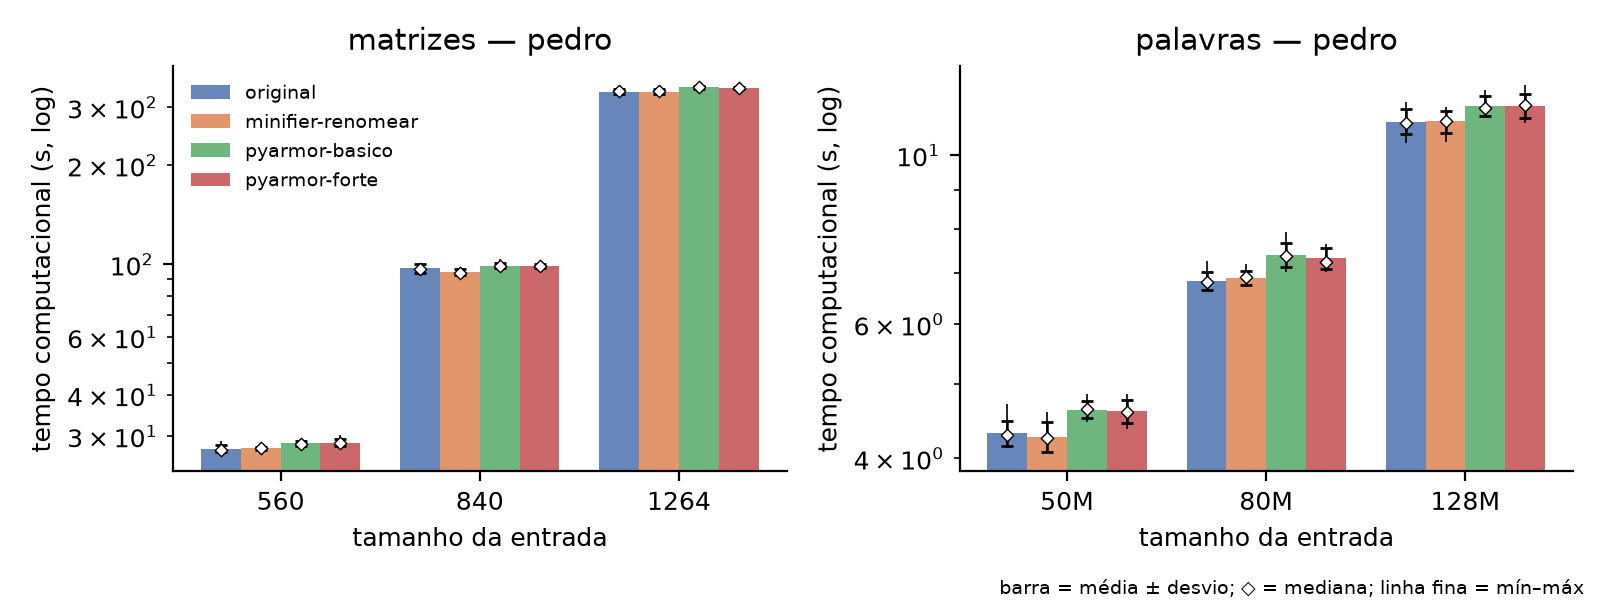
\includegraphics[width=\textwidth]{fig/stats_pedro.png}\\[2pt]
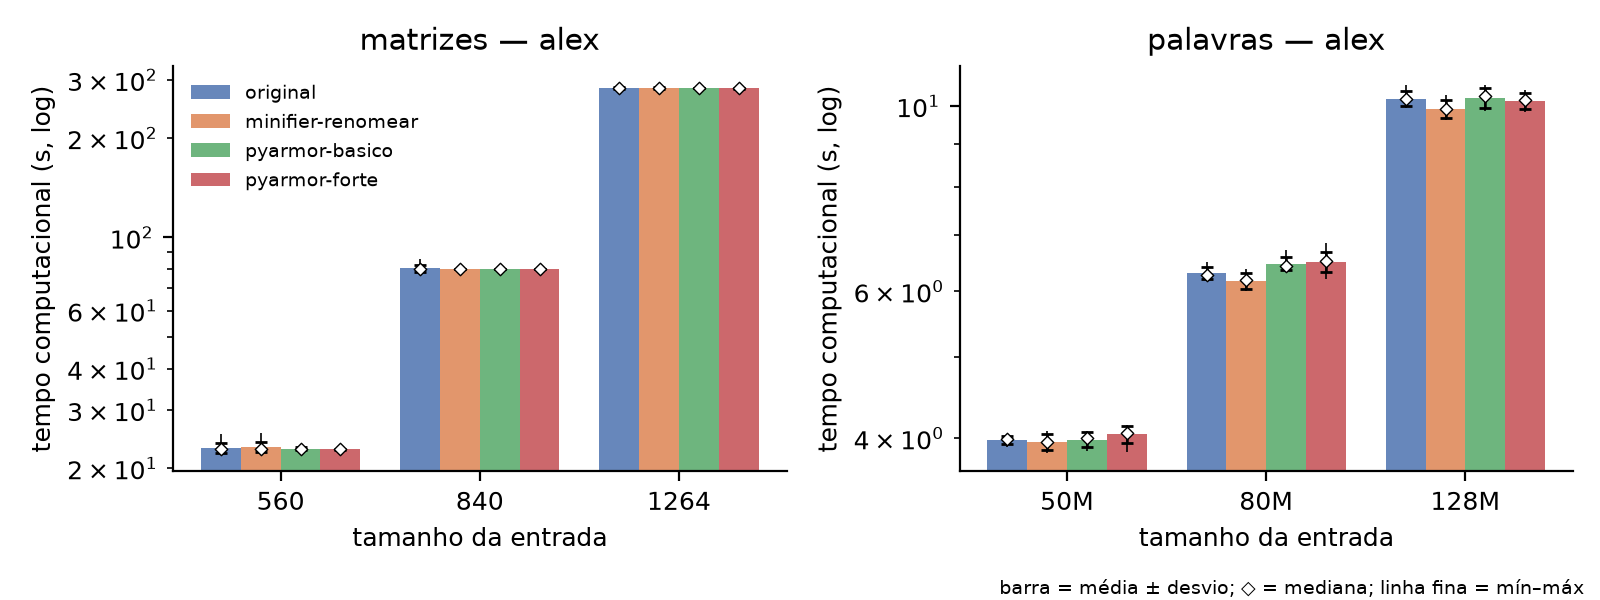
\includegraphics[width=\textwidth]{fig/stats_alex.png}\\[2pt]
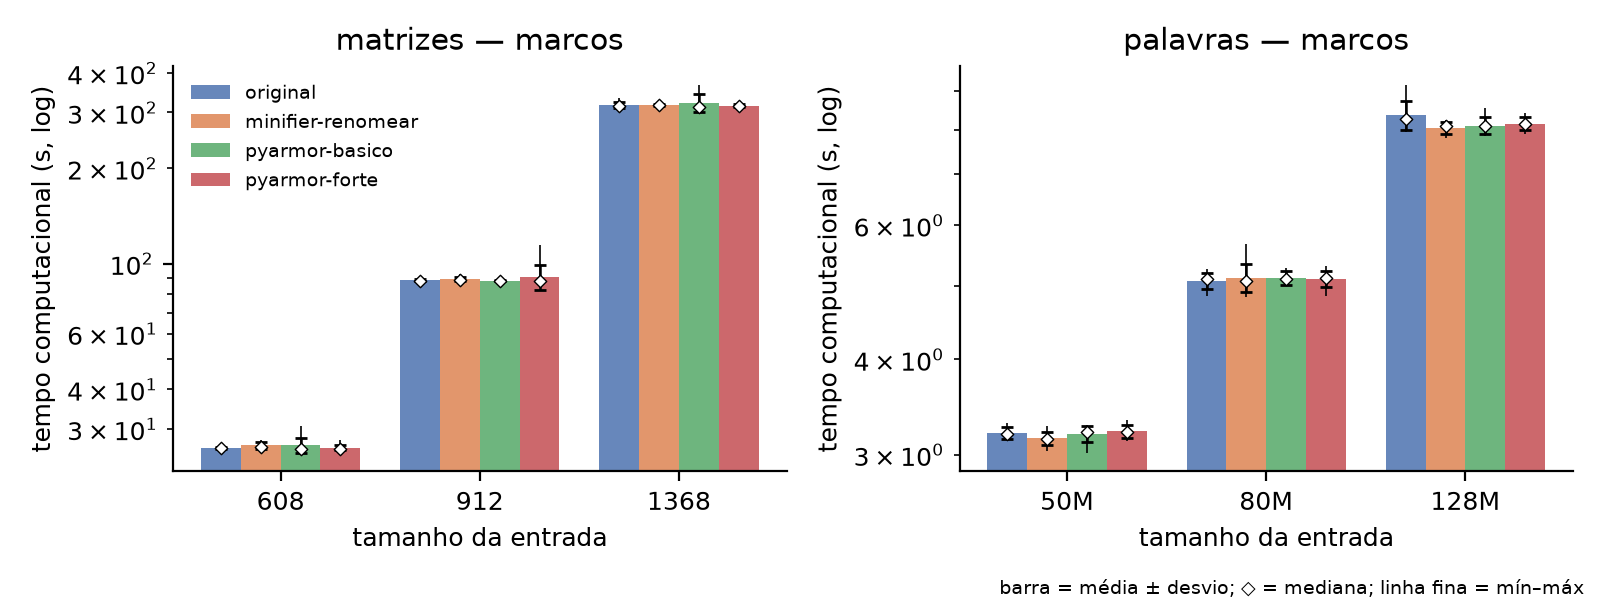
\includegraphics[width=\textwidth]{fig/stats_marcos.png}
\caption{Média $\pm$ desvio padrão (barras), mediana (losango) e mínimo--máximo (traço fino), por máquina, benchmark, tamanho e configuração (escala logarítmica).}\label{fig:stats}
\end{figure}

\begin{table}[ht]\centering\footnotesize
\caption{Matrizes --- máquina Pedro (10 repetições por linha; tempos em s).}\label{tab:pedro-matrizes}
\begin{tabular}{rlrrrrrr}\hline
$n$ & configuração & média & mediana & desvio & mín & máx & slowdown \\\hline
560 & original & 27,464 & 27,275 & 0,653 & 26,659 & 28,993 & 1,000 \\
 & minifier-renomear & 27,553 & 27,663 & 0,331 & 26,933 & 28,023 & 1,003 \\
 & pyarmor-basico & 28,506 & 28,310 & 0,483 & 27,913 & 29,376 & 1,038 \\
 & pyarmor-forte & 28,620 & 28,590 & 0,709 & 27,902 & 30,295 & 1,042 \\
\hline
840 & original & 97,074 & 96,422 & 2,795 & 92,210 & 100,738 & 1,000 \\
 & minifier-renomear & 94,498 & 94,102 & 2,047 & 92,161 & 97,957 & 0,973 \\
 & pyarmor-basico & 98,980 & 98,979 & 1,864 & 96,846 & 103,543 & 1,020 \\
 & pyarmor-forte & 98,861 & 98,909 & 1,503 & 96,778 & 102,081 & 1,018 \\
\hline
1264 & original & 333,784 & 335,045 & 5,784 & 323,321 & 342,395 & 1,000 \\
 & minifier-renomear & 334,618 & 335,580 & 6,919 & 325,628 & 342,407 & 1,002 \\
 & pyarmor-basico & 344,935 & 346,204 & 3,600 & 339,523 & 350,544 & 1,033 \\
 & pyarmor-forte & 343,321 & 343,697 & 2,021 & 340,873 & 346,338 & 1,029 \\
\hline
\end{tabular}\end{table}

\begin{table}[ht]\centering\footnotesize
\caption{Palavras --- máquina Pedro (10 repetições por linha; tempos em s).}\label{tab:pedro-palavras}
\begin{tabular}{rlrrrrrr}\hline
$n$ & configuração & média & mediana & desvio & mín & máx & slowdown \\\hline
50M & original & 4,314 & 4,292 & 0,161 & 4,157 & 4,713 & 1,000 \\
 & minifier-renomear & 4,269 & 4,255 & 0,196 & 4,063 & 4,594 & 0,990 \\
 & pyarmor-basico & 4,633 & 4,640 & 0,118 & 4,469 & 4,858 & 1,074 \\
 & pyarmor-forte & 4,610 & 4,600 & 0,158 & 4,364 & 4,859 & 1,069 \\
\hline
80M & original & 6,833 & 6,809 & 0,185 & 6,660 & 7,272 & 1,000 \\
 & minifier-renomear & 6,900 & 6,913 & 0,147 & 6,720 & 7,189 & 1,010 \\
 & pyarmor-basico & 7,401 & 7,378 & 0,265 & 7,030 & 7,939 & 1,083 \\
 & pyarmor-forte & 7,317 & 7,250 & 0,231 & 7,020 & 7,641 & 1,071 \\
\hline
128M & original & 11,068 & 11,020 & 0,422 & 10,369 & 11,758 & 1,000 \\
 & minifier-renomear & 11,073 & 11,095 & 0,370 & 10,392 & 11,574 & 1,001 \\
 & pyarmor-basico & 11,604 & 11,524 & 0,345 & 11,234 & 12,175 & 1,048 \\
 & pyarmor-forte & 11,619 & 11,634 & 0,424 & 11,019 & 12,369 & 1,050 \\
\hline
\end{tabular}\end{table}

\begin{table}[ht]\centering\footnotesize
\caption{Matrizes --- máquina Alex (10 repetições por linha; tempos em s).}\label{tab:alex-matrizes}
\begin{tabular}{rlrrrrrr}\hline
$n$ & configuração & média & mediana & desvio & mín & máx & slowdown \\\hline
560 & original & 23,046 & 22,788 & 0,821 & 22,690 & 25,372 & 1,000 \\
 & minifier-renomear & 23,161 & 22,898 & 0,843 & 22,797 & 25,549 & 1,005 \\
 & pyarmor-basico & 22,872 & 22,794 & 0,242 & 22,703 & 23,531 & 0,992 \\
 & pyarmor-forte & 22,805 & 22,814 & 0,081 & 22,688 & 22,963 & 0,990 \\
\hline
840 & original & 80,475 & 79,916 & 1,848 & 79,653 & 85,718 & 1,000 \\
 & minifier-renomear & 80,132 & 80,135 & 0,134 & 79,879 & 80,342 & 0,996 \\
 & pyarmor-basico & 80,145 & 80,099 & 0,240 & 79,810 & 80,527 & 0,996 \\
 & pyarmor-forte & 80,132 & 80,141 & 0,166 & 79,883 & 80,463 & 0,996 \\
\hline
1264 & original & 282,548 & 282,243 & 1,830 & 280,048 & 286,012 & 1,000 \\
 & minifier-renomear & 283,539 & 282,820 & 2,290 & 280,526 & 289,233 & 1,004 \\
 & pyarmor-basico & 282,185 & 282,116 & 0,176 & 282,023 & 282,613 & 0,999 \\
 & pyarmor-forte & 282,329 & 282,329 & 0,350 & 281,697 & 282,962 & 0,999 \\
\hline
\end{tabular}\end{table}

\begin{table}[ht]\centering\footnotesize
\caption{Palavras --- máquina Alex (10 repetições por linha; tempos em s).}\label{tab:alex-palavras}
\begin{tabular}{rlrrrrrr}\hline
$n$ & configuração & média & mediana & desvio & mín & máx & slowdown \\\hline
50M & original & 3,974 & 3,990 & 0,043 & 3,900 & 4,013 & 1,000 \\
 & minifier-renomear & 3,955 & 3,954 & 0,086 & 3,837 & 4,076 & 0,995 \\
 & pyarmor-basico & 3,982 & 3,999 & 0,082 & 3,863 & 4,081 & 1,002 \\
 & pyarmor-forte & 4,038 & 4,054 & 0,091 & 3,846 & 4,140 & 1,016 \\
\hline
80M & original & 6,306 & 6,279 & 0,107 & 6,195 & 6,508 & 1,000 \\
 & minifier-renomear & 6,177 & 6,191 & 0,136 & 6,005 & 6,383 & 0,979 \\
 & pyarmor-basico & 6,472 & 6,434 & 0,117 & 6,339 & 6,725 & 1,026 \\
 & pyarmor-forte & 6,509 & 6,528 & 0,180 & 6,202 & 6,856 & 1,032 \\
\hline
128M & original & 10,206 & 10,201 & 0,213 & 9,956 & 10,601 & 1,000 \\
 & minifier-renomear & 9,923 & 9,924 & 0,241 & 9,609 & 10,307 & 0,972 \\
 & pyarmor-basico & 10,227 & 10,268 & 0,270 & 9,851 & 10,592 & 1,002 \\
 & pyarmor-forte & 10,136 & 10,166 & 0,218 & 9,823 & 10,462 & 0,993 \\
\hline
\end{tabular}\end{table}

\begin{table}[ht]\centering\footnotesize
\caption{Matrizes --- máquina Marcos (10 repetições por linha; tempos em s).}\label{tab:marcos-matrizes}
\begin{tabular}{rlrrrrrr}\hline
$n$ & configuração & média & mediana & desvio & mín & máx & slowdown \\\hline
608 & original & 26,175 & 26,045 & 0,244 & 25,986 & 26,584 & 1,000 \\
 & minifier-renomear & 26,676 & 26,242 & 0,680 & 26,053 & 27,786 & 1,019 \\
 & pyarmor-basico & 26,683 & 26,038 & 1,483 & 25,949 & 30,633 & 1,019 \\
 & pyarmor-forte & 26,223 & 26,017 & 0,531 & 25,964 & 27,703 & 1,002 \\
\hline
912 & original & 88,678 & 88,330 & 0,742 & 88,272 & 90,643 & 1,000 \\
 & minifier-renomear & 89,301 & 88,945 & 1,107 & 88,894 & 92,449 & 1,007 \\
 & pyarmor-basico & 88,256 & 88,060 & 0,459 & 87,949 & 89,323 & 0,995 \\
 & pyarmor-forte & 90,741 & 88,054 & 8,277 & 87,979 & 114,289 & 1,023 \\
\hline
1368 & original & 317,464 & 315,249 & 6,591 & 312,588 & 333,673 & 1,000 \\
 & minifier-renomear & 316,474 & 315,683 & 2,624 & 314,218 & 322,920 & 0,997 \\
 & pyarmor-basico & 321,839 & 311,998 & 20,591 & 311,068 & 366,606 & 1,014 \\
 & pyarmor-forte & 315,071 & 314,790 & 3,188 & 310,852 & 319,891 & 0,992 \\
\hline
\end{tabular}\end{table}

\begin{table}[ht]\centering\footnotesize
\caption{Palavras --- máquina Marcos (10 repetições por linha; tempos em s).}\label{tab:marcos-palavras}
\begin{tabular}{rlrrrrrr}\hline
$n$ & configuração & média & mediana & desvio & mín & máx & slowdown \\\hline
50M & original & 3,201 & 3,194 & 0,057 & 3,132 & 3,302 & 1,000 \\
 & minifier-renomear & 3,150 & 3,149 & 0,062 & 3,029 & 3,274 & 0,984 \\
 & pyarmor-basico & 3,196 & 3,209 & 0,075 & 3,014 & 3,279 & 0,998 \\
 & pyarmor-forte & 3,218 & 3,210 & 0,059 & 3,124 & 3,330 & 1,005 \\
\hline
80M & original & 5,069 & 5,093 & 0,126 & 4,851 & 5,255 & 1,000 \\
 & minifier-renomear & 5,117 & 5,063 & 0,218 & 4,831 & 5,666 & 1,009 \\
 & pyarmor-basico & 5,117 & 5,097 & 0,107 & 4,989 & 5,277 & 1,009 \\
 & pyarmor-forte & 5,104 & 5,112 & 0,126 & 4,851 & 5,299 & 1,007 \\
\hline
128M & original & 8,376 & 8,271 & 0,367 & 7,957 & 9,169 & 1,000 \\
 & minifier-renomear & 8,059 & 8,095 & 0,147 & 7,813 & 8,245 & 0,962 \\
 & pyarmor-basico & 8,109 & 8,102 & 0,216 & 7,862 & 8,551 & 0,968 \\
 & pyarmor-forte & 8,149 & 8,152 & 0,160 & 7,906 & 8,421 & 0,973 \\
\hline
\end{tabular}\end{table}


\end{document}
